% Author: Andrej Binovsky <xbinov00@stud.fit.vutbr.cz>
% Author: Zdenek Lapes <xlapes02@stud.fit.vutbr.cz>
% Author: Andrei Shchapaniak <xshcha00@stud.fit.vutbr.cz>
% Author: Richard Gajdosik <xgajdo33@stud.fit.vutbr.cz>


\documentclass[a4paper, 11pt]{article}


\usepackage[slovak]{babel}
\usepackage[utf8]{inputenc}
\usepackage[left=2cm, top=3cm, text={17cm, 24cm}]{geometry}
\usepackage{times}
\usepackage{verbatim}
\usepackage{enumitem}
\usepackage{graphicx} % vkladanie obrazkov
\usepackage[unicode]{hyperref}
\hypersetup{
    colorlinks = false,
    hypertexnames = false,
}

\newcommand{\RNum}[1]{\uppercase\expandafter{\romannumeral #1\relax}} % makro na sázení římských čísel

%%%%%%%%%%%%%%%%%%%%%%%%%%%%%%%% Andrei import -- LL tabulka/pravidla %%%%%%%%%%%%%%%%%%%%%%%%%%%%%%%%

\usepackage{xcolor}
\usepackage{float}
\usepackage{listings}
\usepackage{amsmath}
\usepackage{bm}
\usepackage{makecell}
\usepackage{cprotect}
\usepackage{multirow}
\usepackage{array}
\usepackage{changepage}
\usepackage{color, colortbl}
\definecolor{LightCyan}{rgb}{0.88,1,1}
\definecolor{White}{rgb}{255,255,255}

\def\nonterm #1{\boldmath{$<$}\textbf{#1}\boldmath{$>$}\space}
\def\rot #1{{\rotatebox[origin=c]{90}{\term{#1}}}}
\def\term #1{\texttt{#1}\space}
\newcommand{\arrow} {$\color{red} \rightarrow$\space}
\newcommand{\unsc} {\underline{\hspace{0.2cm}}}
\newcolumntype{P}[1]{>{\centering\arraybackslash}p{#1}}


%%%%%%%%%%%%%%%%%%%%%%%%%%%%%%%% Andrei import -- LL tabulka/pravidla %%%%%%%%%%%%%%%%%%%%%%%%%%%%%%%%

\begin{document}


    %%%%%%%%%%%%%%%%%%%%%%%%%%%%%%%% Titulná stránka %%%%%%%%%%%%%%%%%%%%%%%%%%%%%%%%
    \begin{titlepage}
        \begin{center}
            
\includegraphics[width=0.77\linewidth]{src/FIT_logo.pdf} \\

            \vspace{\stretch{0.382}}

            \Huge{Projektová dokumentácia} \\
            \LARGE{\textbf{Implementácia prekladača imperativného jazyka IFJ21}} \\
            \Large{Tým 082, varianta \RNum{2}}
            \vspace{\stretch{0.618}}
        \end{center}

        \begin{minipage}{0.4 \textwidth}
        {\Large \today}
        \end{minipage}
        \hfill
        \begin{minipage}[r]{0.6 \textwidth}
            \Large
            \begin{tabular}{l l l}
                \textbf{Andrei Shchapaniak} & \textbf{(xshcha00)} & \quad 25\,\% \\
                Andrej Binovsky & (xbinov00) & \quad 25\,\% \\
                Zdenek Lapes & (xlapes02) & \quad 25\,\% \\
                Richard Gajdosik & (xgajdo33) & \quad 25\,\% \\
            \end{tabular}
        \end{minipage}
    \end{titlepage}



    %%%%%%%%%%%%%%%%%%%%%%%%%%%%%%%% Obsah %%%%%%%%%%%%%%%%%%%%%%%%%%%%%%%%
    \pagenumbering{roman}
    \setcounter{page}{1}
    \tableofcontents
    \clearpage



    %%%%%%%%%%%%%%%%%%%%%%%%%%%%%%%% Úvod %%%%%%%%%%%%%%%%%%%%%%%%%%%%%%%%
    \pagenumbering{arabic}
    \setcounter{page}{1}

    \section{Úvod}





    %%%%%%%%%%%%%%%%%%%%%%%%%%%%%%%% Návrh a implementace %%%%%%%%%%%%%%%%%%%%%%%%%%%%%%%%
    \section{Návrh a~implementácia}




    \subsection{Lexikálna analýza}




    \subsection{Syntaktická analýza}



    \subsubsection{Zpracovanie výrazov pomocou precedenčnej syntaktickej analýzy}




    \subsection{Sémantická analýza}




    \subsection{Generovanie cielového kódu}


    \subsubsection{Začiatok generovania}


    \subsubsection{Generovanie -- funkcie}


    \subsubsection{Generovánie -- výrazy}


    \subsubsection{Generovanie -- podmienky a cykly}




    \subsection{Prekladový systém}


    \subsubsection{CMake}



    \subsubsection{GNU Make}




    %%%%%%%%%%%%%%%%%%%%%%%%%%%%%%%% Speciální algoritmy a datové struktury %%%%%%%%%%%%%%%%%%%%%%%%%%%%%%
    \section{Speciálne algoritmy a~dátové štruktúry}

    \subsection{Tabuľka s~rozptýlenými položkami}

    \subsection{Obojsmerný rad}

    \subsection{Zásobník}





    %%%%%%%%%%%%%%%%%%%%%%%%%%%%%%%% Práce v týmu %%%%%%%%%%%%%%%%%%%%%%%%%%%%%%%%
    \section{Práca v~týmu}

    \subsection{Zpôsob práce v~týmu}



    \subsubsection{Verzovací systém}



    \subsubsection{Komunikácia}




    \subsection{Rozdelenie práce mezi členmi týmu}




    %%%%%%%%%%%%%%%%%%%%%%%%%%%%%%%% Závěr %%%%%%%%%%%%%%%%%%%%%%%%%%%%%%%%
    \section{Záver}




    %%%%%%%%%%%%%%%%%%%%%%%%%%%%%%%% Citace %%%%%%%%%%%%%%%%%%%%%%%%%%%%%%%%
    \clearpage
    \bibliographystyle{czechiso}
    \renewcommand{\refname}{Literatura}
    \bibliography{dokumentace}



    %%%%%%%%%%%%%%%%%%%%%%%%%%%%%%%% Přílohy %%%%%%%%%%%%%%%%%%%%%%%%%%%%%%%%
    \clearpage


    %%%%%%%%%%%%%%%%%%%%%%%%%%%%%%%% Diagram konečného automatu %%%%%%%%%%%%%%%%%%%%%%%%%%%%%%%%

    \section*{Diagram konečného automatu specifikujúceho lexikálny analyzátor}
    \begin{figure}[!ht]
        \centering
        \vspace{-1.2cm}
        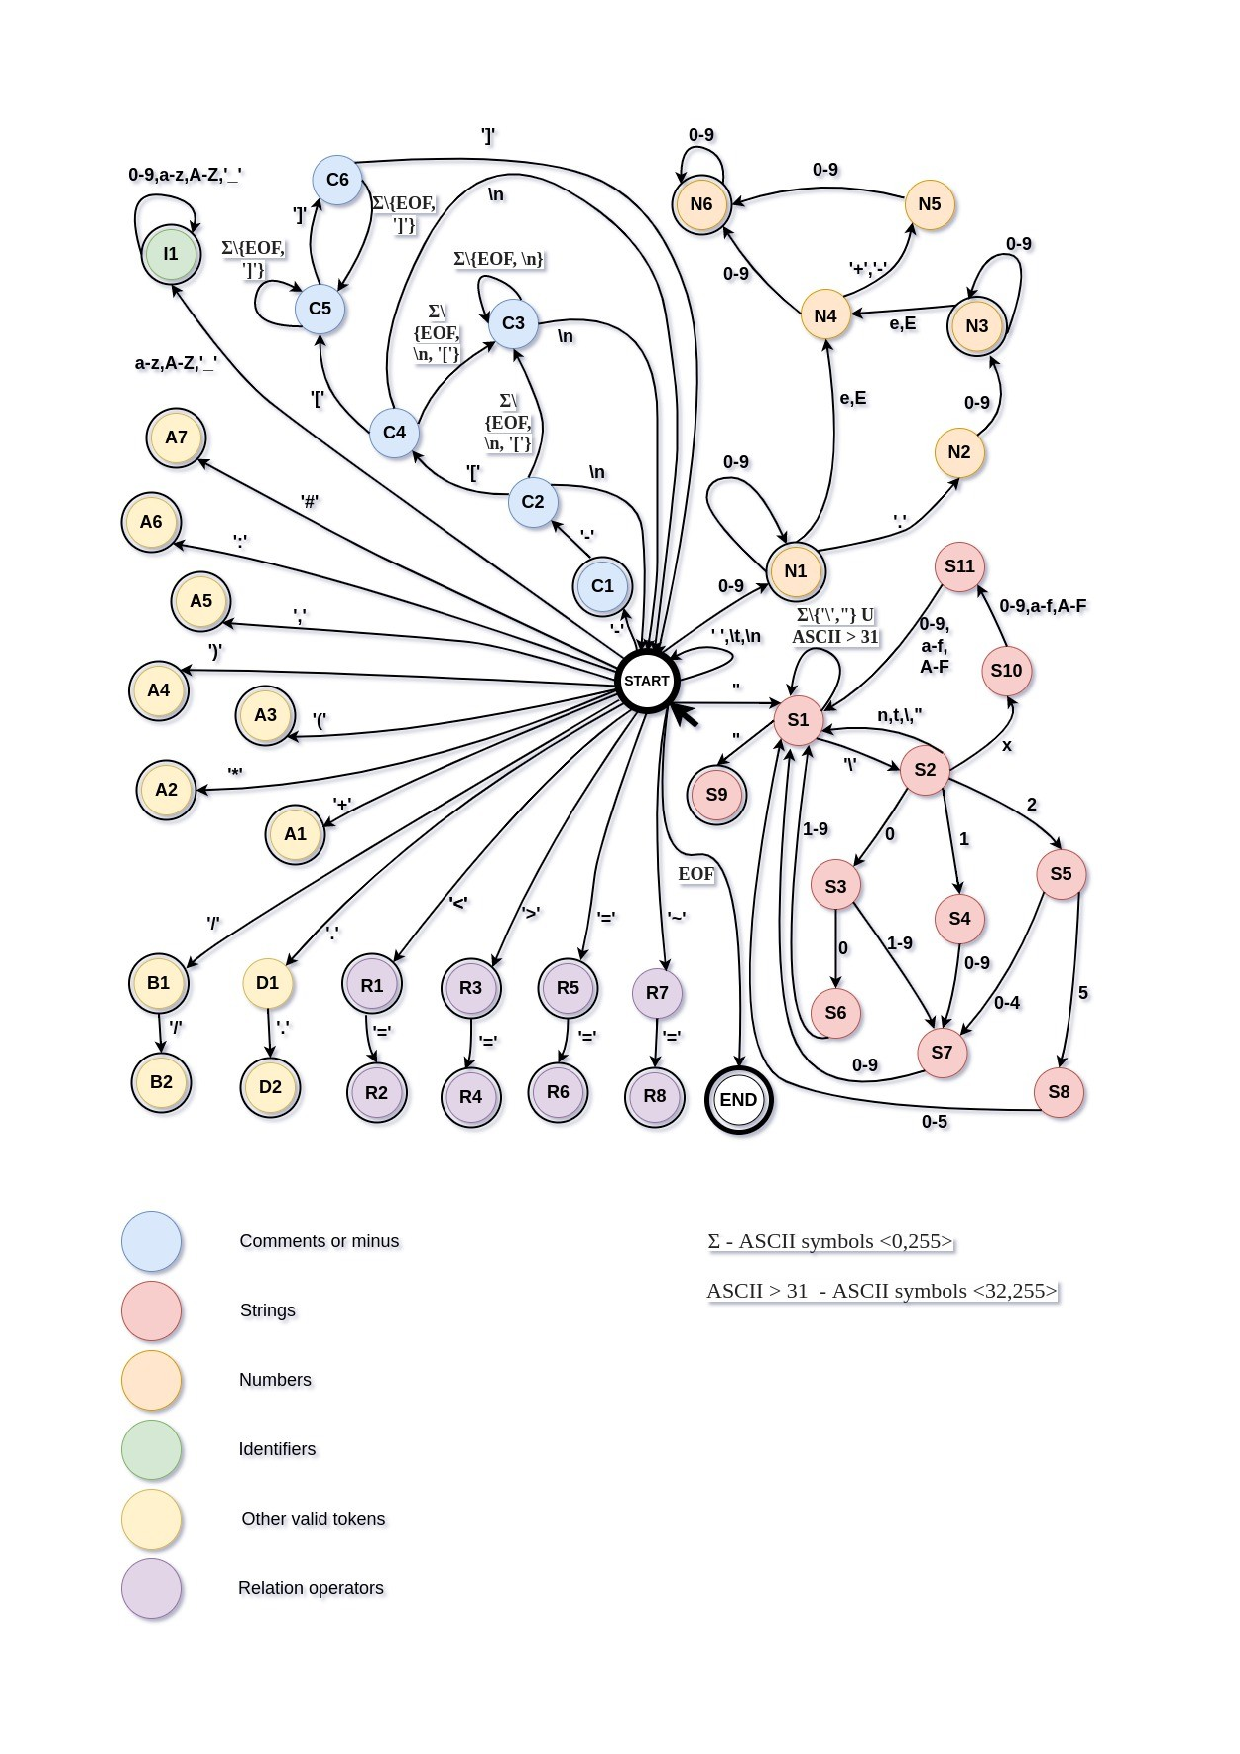
\includegraphics[width=0.95\linewidth]{src/FSM_PDF.pdf}
        \caption{Diagram konečného automatu specifikující lexikální analyzátor}
        \label{figure:fa_graph}
    \end{figure}

    %%%%%%%%%%%%%%%%%%%%%%%%%%%%%%%% LL -- gramatika %%%%%%%%%%%%%%%%%%%%%%%%%%%%%%%%
    \section*{LL -- gramatika}
    \begin{enumerate}[label=\textcolor{red}{\arabic*.}]
        \item \nonterm{prolog} \arrow{} \term{require} \term{t\unsc{}string} \nonterm{prog}

        \item \nonterm{prog} \arrow{} \term{global} \term{id} \term{:} \term{function} \term{(} \nonterm{arg\unsc{}T} \term{)} \nonterm{ret\unsc{}T} \nonterm{prog}

        \item \nonterm{prog} \arrow{} \term{function} \term{id} \term{(} \nonterm{arg} \term{)} \nonterm{ret\unsc{}T} \nonterm{stmt} \term{end} \nonterm{prog}

        \item \nonterm{prog} \arrow{} \term{id} \term{(} \nonterm{param} \term{)} \nonterm{prog}
        \item \nonterm{prog} \arrow{} \term{EOF}

        \item \nonterm{arg\unsc{}T} \arrow{} \nonterm{type} \nonterm{next\unsc{}arg\unsc{}T}
        \item \nonterm{arg\unsc{}T} \arrow{} \term{$\varepsilon$}

        \item \nonterm{next\unsc{}arg\unsc{}T} \arrow{} \term{,} \nonterm{type} \nonterm{next\unsc{}arg\unsc{}T}

        \item \nonterm{next\unsc{}arg\unsc{}T} \arrow{} \term{$\varepsilon$}

        \item \nonterm{ret\unsc{}T} \arrow{} \term{:} \nonterm{type} \nonterm{next\unsc{}ret\unsc{}T}

        \item \nonterm{ret\unsc{}T} \arrow{} \term{$\varepsilon$}

        \item \nonterm{next\unsc{}ret\unsc{}T} \arrow{} \term{,} \nonterm{type} \nonterm{next\unsc{}ret\unsc{}T}

        \item \nonterm{next\unsc{}ret\unsc{}T} \arrow{} \term{$\varepsilon$}

        \item \nonterm{arg} \arrow{} \term{id} \term{:} \nonterm{type} \nonterm{next\unsc{}arg}
        \item \nonterm{arg} \arrow{} \term{$\varepsilon$}

        \item \nonterm{next\unsc{}arg} \arrow{} \term{,} \term{id} \term{:} \nonterm{type} \nonterm{next\unsc{}arg}

        \item \nonterm{next\unsc{}arg} \arrow{} \term{$\varepsilon$}

        \item \nonterm{type} \arrow{} \term{integer}
        \item \nonterm{type} \arrow{} \term{number}
        \item \nonterm{type} \arrow{} \term{string}
        \item \nonterm{type} \arrow{} \term{nil}

        \item \nonterm{stmt} \arrow{} \term{if} \nonterm{expr} \term{then} \nonterm{stmt} \term{else} \nonterm{stmt} \term{end} \nonterm{stmt}

        \item \nonterm{stmt} \arrow{} \term{while} \nonterm{expr} \term{do} \nonterm{stmt} \term{end} \nonterm{stmt}

        \item \nonterm{stmt} \arrow{} \term{local} \term{id} \term{:} \nonterm{type} \nonterm{def\unsc{}var} \nonterm{stmt}

        \item \nonterm{stmt} \arrow{} \term{return} \nonterm{expr} \nonterm{next\unsc{}expr} \nonterm{stmt}

        \item \nonterm{stmt} \arrow{} \term{id} \nonterm{fork\unsc{}id} \nonterm{stmt}

        \item \nonterm{stmt} \arrow{} \term{$\varepsilon$}

        \item \nonterm{def\unsc{}var} \arrow{} \term{=} \nonterm{one\unsc{}assign}
        \item \nonterm{def\unsc{}var} \arrow{} \term{$\varepsilon$}

        \item \nonterm{one\unsc{}assign} \arrow{} \term{id} \term{(} \nonterm{param} \term{)}
        \item \nonterm{one\unsc{}assign} \arrow{} \nonterm{expr}

        \item \nonterm{param} \arrow{} \nonterm{param\unsc{}val} \nonterm{next\unsc{}param}
        \item \nonterm{param} \arrow{} \term{$\varepsilon$}

        \item \nonterm{param\unsc{}val} \arrow{} \term{id}
        \item \nonterm{param\unsc{}val} \arrow{} \nonterm{term}

        \item \nonterm{term} \arrow{} \term{t\unsc{}string}
        \item \nonterm{term} \arrow{} \term{t\unsc{}integer}
        \item \nonterm{term} \arrow{} \term{t\unsc{}number}
        \item \nonterm{term} \arrow{} \term{nil}

        \item \nonterm{next\unsc{}param} \arrow{} \term{,} \nonterm{param\unsc{}val} \nonterm{next\unsc{}param}

        \item \nonterm{next\unsc{}param} \arrow{} \term{$\varepsilon$}

        \item \nonterm{next\unsc{}expr} \arrow{} \term{,} \nonterm{expr} \nonterm{next\unsc{}expr}
        \item \nonterm{next\unsc{}expr} \arrow{} \term{$\varepsilon$}

        \item \nonterm{fork\unsc{}id} \arrow{} \term{(} \nonterm{param} \term{)}
        \item \nonterm{fork\unsc{}id} \arrow{} \nonterm{next\unsc{}id}

        \item \nonterm{next\unsc{}id} \arrow{} \term{,} \term{id} \nonterm{next\unsc{}id}
        \item \nonterm{next\unsc{}id} \arrow{} \term{=} \nonterm{mult\unsc{}assign}

        \item \nonterm{mult\unsc{}assign} \arrow{} \term{id} \term{(} \nonterm{param} \term{)}
        \item \nonterm{mult\unsc{}assign} \arrow{} \nonterm{expr} \nonterm{next\unsc{}expr}
    \end{enumerate}

    %%%%%%%%%%%%%%%%%%%%%%%%%%%%%%%% LL -- tabulka %%%%%%%%%%%%%%%%%%%%%%%%%%%%%%%%
    \newpage
    \section*{LL -- tabulka}

    \begin{table}[htb]
        \begin{adjustwidth}{-0.2cm}{}
            \begin{tabular}{!{\vrule width 2pt}>{\columncolor{LightCyan}}P{2.3cm}!{\vrule width 2pt}P{2.5mm}|P{2.5mm}|P{2.5mm}|P{2.5mm}|P{2.5mm}|P{2.5mm}|P{2.5mm}|P{2.5mm}|P{2.5mm}|P{2.5mm}|P{2.5mm}|P{2.5mm}|P{2.5mm}|P{2.5mm}|P{2.5mm}|P{2.5mm}|P{2.5mm}|P{2.5mm}|P{2.5mm}|P{2.5mm}|P{2.5mm}!{\vrule width 2pt}}
                \Xhline{5\arrayrulewidth} \rowcolor{LightCyan}
                \cellcolor{White}& \rot{require} & \rot{global} & \rot{function} & \rot{id} & \rot{integer}
                & \rot{string} & \rot{number} & \rot{nil} & \rot{t\unsc{}integer} & \rot{t\unsc{number}} & \rot{t\unsc{}string} & \rot{if} & \rot{while} & \rot{local} & \rot{return}  & \rot{:} & \rot{=} & \rot{(} & \rot{,} & \rot{EOF} & \rot{\$}\\
                \Xhline{5\arrayrulewidth}
                \nonterm{prolog} & 1 & & & & & & & & & & & & & & & & & & & & \\
                \hline
                \nonterm{prog} & & 2 & 3 & 4 & & & & & & & & & & & & & & & & 5 &\\
                \hline
                \nonterm{arg\unsc{}T} & & & & & 6 & 6 & 6 & 6 & & & & & & & & & & & & & 7 \\
                \hline
                \nonterm{next\unsc{}arg\unsc{}T} & & & & & & & & & & & & & & & & & & & 8 & & 9 \\
                \hline
                \nonterm{ret\unsc{}T} & & & & & & & & & & & & & & & & 10 & & & & & 11 \\
                \hline
                \nonterm{next\unsc{}ret\unsc{}T} & & & & & & & & & & & & & & & & & & & 12 & & 13 \\
                \hline
                \nonterm{arg} & & & & 14 & & & & & & & & & & & & & & & & & 15 \\
                \hline
                \nonterm{next\unsc{}arg} & & & & & & & & & & & & & & & & & & & 16 & & 17 \\
                \hline
                \nonterm{type} & & & & & 18 & 20 & 19 & 21 & & & & & & & & & & & & &\\
                \hline
                \nonterm{stmt} & & & & 26 & & & & & & & & 22 & 23 & 24 & 25 & & & & & & 27 \\
                \hline
                \nonterm{def\unsc{}var} & & & & & & & & & & & & & & & & & 28 & & & & 29 \\
                \hline
                \nonterm{one\unsc{}assign} & & & & 30 & & & & & & & & & & & & & & & & & 31 \\
                \hline
                \nonterm{param} & & & & 32 & & & & 32 & 32 & 32 & 32 & & & & & & & & & & 33 \\
                \hline
                \nonterm{param\unsc{}val} & & & & 34 & & & & 35 & 35 & 35 & 35 & & & & & & & & & &\\
                \hline
                \nonterm{term} & & & & & & & & 39 & 37 & 38 & 36 & & & & & & & & & &\\
                \hline
                \nonterm{next\unsc{}param} & & & & & & & & & & & & & & & & & & & 40 & & 41 \\
                \hline
                \nonterm{next\unsc{}expr} & & & & & & & & & & & & & & & & & & & 42 & & 43\\
                \hline
                \nonterm{fork\unsc{}id} & & & & & & & & & & & & & & & & & 45 & 44 & 45 & & \\
                \hline
                \nonterm{next\unsc{}id} & & & & & & & & & & & & & & & & & 47 & & 46 & & \\
                \hline
                \nonterm{mult\unsc{}assign} & & & & 48 & & & & & & & & & & & & & & & & & 49 \\
                \hline
                \Xhline{5\arrayrulewidth}
            \end{tabular}
        \end{adjustwidth}
    \end{table}


    %%%%%%%%%%%%%%%%%%%%%%%%%%%%%%%% PRECEDENCNI TABULKA %%%%%%%%%%%%%%%%%%%%%%%%%%%%%%%%
    \newpage
    \section*{Precedenčná tabuľka}
    \newcommand{\bE}{\textbf{E}}
    \begin{table}[!htbp]
        \centering
        \begin{tabular}{l@{\hskip 1in} l@{\hskip 1in} l}
            $\color{red} 1.$ \bE{} \space\arrow{} i               & $\color{red} 6.$  \bE{} \space\arrow{} \bE{} $*$ \bE{}  & $\color{red} 11.$ \bE{} \space\arrow{} \bE{} $<$ \bE{}     \\
            $\color{red} 2.$ \bE{} \space\arrow{} ( \bE{} )         & $\color{red} 7.$  \bE{} \space\arrow{} \bE{} $/$ \bE{}  & $\color{red} 12.$ \bE{} \space\arrow{} \bE{} $>=$ \bE{}    \\
            $\color{red} 3.$ \bE{} \space\arrow{} \# \bE{}         & $\color{red} 8.$  \bE{} \space\arrow{} \bE{} $//$ \bE{} & $\color{red} 13.$ \bE{} \space\arrow{} \bE{} $<=$ \bE{}    \\
            $\color{red} 4.$ \bE{} \space\arrow{} \bE{} $+$ \bE{} & $\color{red} 9.$  \bE{} \space\arrow{} \bE{} .. \bE{}   & $\color{red} 14.$ \bE{} \space\arrow{} \bE{} $==$ \bE{}    \\
            $\color{red} 5.$ \bE{} \space\arrow{} \bE{} $-$ \bE{} & $\color{red} 10.$ \bE{} \space\arrow{} \bE{} $>$ \bE{}  & $\color{red} 15.$ \bE{} \space\arrow{} \bE{} $\sim=$ \bE{} \\
        \end{tabular}
    \end{table}

    \begin{center}
        \begin{adjustwidth}{-0.4cm}{}
            \begin{tabular}{!{\vrule width 2pt} >{\columncolor{LightCyan}}P{5.5mm} !{\vrule width 2pt} P{5.5mm} | P{5.5mm} | P{5.5mm} | P{5.5mm} | P{5.5mm} | P{5.5mm} | P{5.5mm} | P{5.5mm} | P{5.5mm} | P{5.5mm} | P{5.5mm} | P{5.5mm} | P{5.5mm} | P{5.5mm} | P{5.5mm} | P{5.5mm} | P{5.5mm} !{\vrule width 2pt}}
                \Xhline{5\arrayrulewidth}\rowcolor{LightCyan}
                \cellcolor{White}& \textbf{\#} & \textbf{*} & \textbf{/} & \textbf{//} & \textbf{+} & \textbf{-} & \textbf{..} & $\bm{<}$ & $\bm{<=}$ & $\bm{>}$ & $\bm{>=}$ & $\bm{==}$ & $\bm{\sim=}$ & \textbf{(} & \textbf{)} & \textbf{i} & \textbf{\$} \\ [0.6ex]
                \Xhline{5\arrayrulewidth}
                \textbf{\#}      & $<$ & $>$ & $>$ & $>$ & $>$ & $>$ & $>$ & $>$ & $>$ & $>$ & $>$ & $>$ & $>$ & $<$ & $>$ & $<$ & $>$ \\ [0.5ex]
                \hline
                \textbf{*}       & $<$ & $>$ & $>$ & $>$ & $>$ & $>$ & $>$ & $>$ & $>$ & $>$ & $>$ & $>$ & $>$ & $<$ & $>$ & $<$ & $>$ \\ [0.5ex]
                \hline
                \textbf{/}       & $<$ & $>$ & $>$ & $>$ & $>$ & $>$ & $>$ & $>$ & $>$ & $>$ & $>$ & $>$ & $>$ & $<$ & $>$ & $<$ & $>$ \\ [0.5ex]
                \hline
                \textbf{//}      & $<$ & $>$ & $>$ & $>$ & $>$ & $>$ & $>$ & $>$ & $>$ & $>$ & $>$ & $>$ & $>$ & $<$ & $>$ & $<$ & $>$ \\ [0.5ex]
                \hline
                \textbf{+}       & $<$ & $<$ & $<$ & $<$ & $>$ & $>$ & $>$ & $>$ & $>$ & $>$ & $>$ & $>$ & $>$ & $<$ & $>$ & $<$ & $>$ \\ [0.5ex]
                \hline
                \textbf{-}       & $<$ & $<$ & $<$ & $<$ & $>$ & $>$ & $>$ & $>$ & $>$ & $>$ & $>$ & $>$ & $>$ & $<$ & $>$ & $<$ & $>$ \\ [0.5ex]
                \hline
                \textbf{..}      & $<$ & $<$ & $<$ & $<$ & $<$ & $<$ & $<$ & $>$ & $>$ & $>$ & $>$ & $>$ & $>$ & $<$ & $>$ & $<$ & $>$ \\ [0.5ex]
                \hline
                $\bm{<}$     & $<$ & $<$ & $<$ & $<$ & $<$ & $<$ & $<$ & $>$ & $>$ & $>$ & $>$ & $>$ & $>$ & $<$ & $>$ & $<$ & $>$ \\ [0.5ex]
                \hline
                $\bm{<=}$    & $<$ & $<$ & $<$ & $<$ & $<$ & $<$ & $<$ & $>$ & $>$ & $>$ & $>$ & $>$ & $>$ & $<$ & $>$ & $<$ & $>$ \\ [0.5ex]
                \hline
                $\bm{>}$     & $<$ & $<$ & $<$ & $<$ & $<$ & $<$ & $<$ & $>$ & $>$ & $>$ & $>$ & $>$ & $>$ & $<$ & $>$ & $<$ & $>$ \\ [0.5ex]
                \hline
                $\bm{>=}$    & $<$ & $<$ & $<$ & $<$ & $<$ & $<$ & $<$ & $>$ & $>$ & $>$ & $>$ & $>$ & $>$ & $<$ & $>$ & $<$ & $>$ \\ [0.5ex]
                \hline
                $\bm{==}$    & $<$ & $<$ & $<$ & $<$ & $<$ & $<$ & $<$ & $>$ & $>$ & $>$ & $>$ & $>$ & $>$ & $<$ & $>$ & $<$ & $>$ \\ [0.5ex]
                \hline
                $\bm{\sim=}$ & $<$ & $<$ & $<$ & $<$ & $<$ & $<$ & $<$ & $>$ & $>$ & $>$ & $>$ & $>$ & $>$ & $<$ & $>$ & $<$ & $>$ \\ [0.5ex]
                \hline
                \textbf{(}       & $<$ & $<$ & $<$ & $<$ & $<$ & $<$ & $<$ & $<$ & $<$ & $<$ & $<$ & $<$ & $<$ & $<$ & $=$ & $<$ &  e  \\ [0.5ex]
                \hline
                \textbf{)}       & $>$ & $>$ & $>$ & $>$ & $>$ & $>$ & $>$ & $>$ & $>$ & $>$ & $>$ & $>$ & $>$ &  e  & $>$ &  s  & $>$ \\ [0.5ex]
                \hline
                \textbf{i}       &  e  & $>$ & $>$ & $>$ & $>$ & $>$ & $>$ & $>$ & $>$ & $>$ & $>$ & $>$ & $>$ &  e  & $>$ &  s  & $>$ \\ [0.5ex]
                \hline
                \textbf{\$}      & $<$ & $<$ & $<$ & $<$ & $<$ & $<$ & $<$ & $<$ & $<$ & $<$ & $<$ & $<$ & $<$ & $<$ &  e  & $<$ &  e  \\ [0.5ex]
                \Xhline{5\arrayrulewidth}
            \end{tabular}
        \end{adjustwidth}
    \end{center}

    LEGENDA: \\
    $<$  \space-\space insert to stack with shift \\
    $>$  \space-\space reduction \\
    =    \space-\space insert to stack \\
    e    \space-\space error \\
    s    \space-\space special case (end of expression)\\


\end{document}
